\section{Text Normalisation Techniques}
\label{sec-background}

\subsection{Text Pruning}
Before we begin analysing our tokens, we would want to categorise and extract the tokens which we would want to consider for Normalisation. Our focus is to segregate out tokens into various categories, such as In Vocabulary, Non Candidates and Out of Vocabulary text. We use $labelled-tweets.txt$ for extracting the labelled tokens using $listing.py$. This gives us tokens in a line-by-line format. 


\texttt {\citet{lnt15b}} tokenises and classifies strings into three main categories In-Vocabulary, Out of Vocabulary $($$OOV$$)$ and Non candidate tokens ($NO$). For the purpose of out study, we run a Levenshtein difference analysis using $distance.py$ and place tokens with difference 0 into in-vocabulary terms. The Levenshtein distance is calculated as per the number of substitutions, deletions or additions to be made to the input string to convert the string ${L}$ to ${D}$. 

In order to identify non-candidates (NO), we run a regex string check, on all the terms to classify strings beginning with punctuation symbols, character {\nolinkurl{@}} or \# or http websites using $Outliers.py$. Thus, candidates without the presence of in vocabulary terms and special characters are marked as candidates for lexical normalisation and are termed Out-of-Vocabulary (OOV). 

Usually these are terms that have been misspelt of have been abbreviated in order to fit Twitters 140 character limit. Our $results.txt$ document now contains all the IN and NO words up till this point. For the remaining candidates we perform the normalisation techniques.  \textbf{Table 1} represents the corpura of the words we have used for normalisation. 

\subsection{{\itshape LRPN} Technique}
\begin{table}[t]
\centering

 \begin{tabular}{|c|c|} 
 \hline
 Corpus & Features \\ [0.5ex] 
 \hline\hline
 labelled-tweets.txt & 53KB \\ 
\hline
labelled-tokens.txt & 127KB \\
 \hline
 tokens.txt & 49 KB (8841 words) \\
 \hline
\end{tabular}
\mycaption{Corpura used for Normalisation
\label{tbl-normalize}}
\aftertabspace
\end{table}
  
 \textbf{Normalisation Process:}
  
\textbf{Calculating Edit Distance:} First, the terms with edit distance of 2 are identified and results are stored in an array. These contain words based textual similarity. For this, we use the python-Levenshtein 0.12.0 package. The phrase edit distance is used 
  to refer specifically to Levenshtein distance.The dictionary terms (dict.txt) is searched for matches based on Levenshtein Distance. We perform this step through $distance.py$ and segregate our input token strings $dictionary words$ and $non dictionary$ words. 
  
 \textbf {Note:} Although it is possible to retrace the dictionary words corresponding to the lowest value of the edit distance, we take a conscious decision, based on evaluation of several edit distance measures (global and local) on not doing so as the accuracy of these words extracted will not be optimal in most cases. Subsequently, we combine several techniques to approach the same.
    
\textbf{Peter Norvig's Algorithm:} {\citet{pn15}} introduced an algorithm for the approximate matches. This returns one match deemed closest to the query by the algorithm. Peter Norwig's algorithm considers corrections that require two simple edits. The following steps are performed: Selection Mechanism, Candidate Model, Language Model and Error Model. We use $PeterNorwig.py$ for evaluating the Peter Norwig correction. We combine Peter Norvig with N-gram context matching for increasing the accuracy of normalisation.
  
\textbf{N-gram matching:} $n-gram$ is a contiguous sequence of n items is analysed from a given sequence of text or speech. An n-gram of size 1 is referred to as a "unigram"; size 2 is a "bigram" (or, less commonly, a "digram"); size 3 is a "trigram". Larger sizes are sometimes referred to by the value of n in modern language, e.g., "four-gram", "five-gram", and so on. 
   
   
For each of the OOV's we run different $n-gram$ values from $N=1$ to $N=5$ values using ${generate}\textunderscore{resultsimilarity}.py$. We do this as n-gram may not give us the appropriate string match for lower values of ngram. Through this we analyse the best  ngram decimal values we have obtained for each of the OOV tokens and use ${gen}\textunderscore {nresult.py}$, to pull out the highest ngram value corresponding to each word. For instance, say the OOV word 'commig', the value we get for $N=1$ is $0.875000000$ and the value for $N=2$ is $0.888888889$.

We further maintain a list of all the best N-values for each word and maintain a 
count using ${gennhighest.py}$. From this we make a deduction to find what is the most occurring value of N, giving us the highest results and we further use our chosen N-value to backtrack the possible dictionary word. We use ${gen}
\textunderscore{correspondword.py}$ for getting the possible dictionary word.

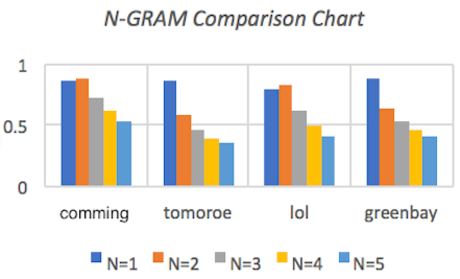
\includegraphics {finalgraph4.pdf}
   
\subsection{{\itshape NLTK-SRI} Technique}

{\citet{gmctw14}} first conduct a context free analysis (at the linguistic level) of all the non-English words. Thus terms such as '2day', 'today' are consider distinct words. Next, they perform normalisation on the noisy text to recover the surface form of the message and record the contextual dimensions, such as, client and location. A text cleaner is built to handle morphophonemic variations. The cleanser marks @username with *USR* and hashtags that are preceded before the end of messages are removed. Hashtags within the middle of the word are removed.

Next, NLTK tokeniser is used to split all tokens that include punctuation symbols. (\textbackslash$w$\text{*}) $($$[$ $P$$]$$)$ (\textbackslash$w$\text{*}) $\rightarrow$ $[$\textbackslash$1$,\textbackslash$2$,\textbackslash$3$$]$ can be used for the same. A confusion network $CN$ is built by comparing token to the words in lexicon $L$. All the tokens be it $IN$ or $OOV$ or punctuation is added tot the CN with probability 1.0. Under the data directory $common\textunderscore abbrs.csv$ maintain a for optimising referencing. A transliteration look up table is built to convert text such as 't0day' $\rightarrow$ ['t0day','today'],refer \textbf{Table 2}. Ranking is performed through a heuristic function (sim()) for each candidate word. 

Confusion Set that is produced this way is joined with the previous set. Finally, lattice is decodes with the use of probabilistic finite state grammar format. At this point, SRI-LM's $lattice-tool$ is used to find the best path through the lattice and training of the set is done as follows. For selecting clean tweets, the following measure was used. Lastly, training of 30M words is done on this set.

\begin{equation}
\label{eq:pr}
\frac{\mathit{Number\ of\ OOV}}{\mathit{Number\ of\ IV+1}} < P ; where P=0.5.
\end{equation}


\begin{table}[t]
\centering

 \begin{tabular}{c c c c} 
 \hline
 Character & Transliteration candidates \\ [0.5ex] 
 \hline\hline
 1 & '1','1','one' \\ 

 2 & '2','to','too','two' \\

 3 & '3','e','three'\\

 4 & '4','a','for','four' \\
 
 5 & '5','s','five' \\ 

 6 & '6','b','six' \\

 7 & '7','t','seven'\\

 8 & '8','ate','eight' \\
 
 9 & '9','g','nine' \\ 

 0 & '0','o','zero' \\

 '@' & '@','at'\\

 "\&" & '\&','and' \\

 \hline
\end{tabular}
\mycaption{Transiliteration lookup table
\label{tbl-normalize}}
\aftertabspace
\end{table}
  










  
